\cc{\chapter{Evaluation of the original application}}
\renewcommand{\baselinestretch}{\mystretch}
\label{chap:Eval}
%\setlength{\parindent}{0pt}

\ca{\section{Example sequences}}

\PARstart{\ca{A}}{} \ca{few existing sequence designs used for past lighting shows were available for use as example inputs. They all share the same set of output controller \cc{configurations}. The longest sequence\cc{,} with a mixture of \cc{slowly} and \cc{rapidly} changing effects\cc{,} was used for all subsequent performance analysis to represent \cc{the both types} of lighting show designs \cc{complexities}. \fref{fig:diff} shows the complexity of this test sequence, plotted by averaging the percentage difference between two continuous frames every second. This sequence lasts for 6 minutes and 49 seconds. \cb{It was made from} 2900 elements\cb{, a total of} 8452 output channels.
}

\begin{figure}[!t]
  \centering
  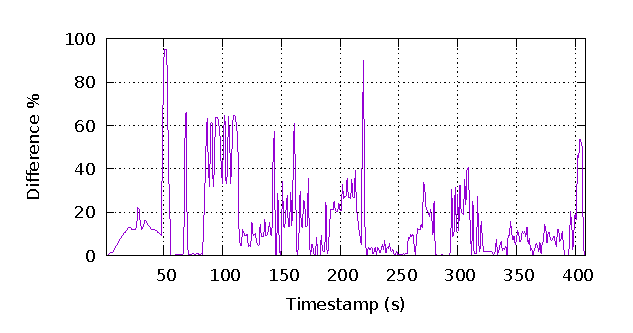
\includegraphics[width=0.8\columnwidth]{Figs/diff.eps}
  \caption{\footnotesize Frame difference of the test sequence averaged every second}
  \label{fig:diff}
\end{figure}

\section{Original performance}

The original Vixen application already has \ca{a} built-in instrumentation display interface that can show runtime performance figures such as controller update speeds. However, it lacks some elemental functionalities for performance analysis. Data logging, playback timestamps and CPU usage logging were added for performance analysis.

The Vixen application uses a separate thread for each task. It has the main GUI thread for \cc{the} editor, a preview rendering thread and multiple dedicated threads for active controllers. This multi-threading structure can take advantage of modern multi-core multi-thread processors. However, performance on a \cc{single-core} machine can be poor due to context switching. Mutex locks are also required to resolve potential data access \cc{conflicts}, further \ca{increasing} the overhead.

\begin{figure}[!t]
  \centering
  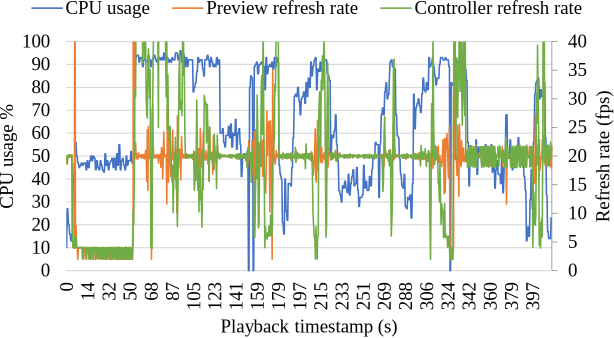
\includegraphics[width=0.8\columnwidth]{original}
  \caption{\footnotesize Performance of original Vixen execution engine}
  \label{fig:original}
\end{figure}

\fref{fig:original} shows the performance of the original Vixen execution engine \ca{on the Microsoft Windows-based platform}. The CPU usage frequently \ca{reached} above $90 \%$ \ca{when the sequence complexity increases}, while the refresh rate \ca{was} very unstable around the configured 20 fps. Especially \ca{during} the first 60 seconds, the refresh rate \ca{dropped} to 5 fps while trying to keep up with element updates. At the same time, the CPU usage was \ca{around} $50 \%$. On a dual-core machine, this implies one of the cores was running at full load while the other one was mostly idle.

Further analysis using Microsoft Visual Studio's sampling profiler shows around $24.7 \%$ of total CPU time was \ca{spent} between translation layers for generating controller commands (\texttt{GenerateCommand}), while the actual command assignment (\texttt{\_8BitEvaluator}) \ca{took} less than $0.5 \%$ of CPU time, as shown \ca{in} \fref{fig:vixen_perf_original}'s \ca{call tree} analysis. Another $23.0 \%$ \cc{of} CPU time was used for filter and element updates, $26.0 \%$ for preview rendering and $16.9 \%$ for the sequence editor, as shown \ca{in} \fref{fig:vixen_perf_original_overview}. The CPU time used for controller updates \ca{was} almost negligible.

\begin{figure}[!t]
  \centering
  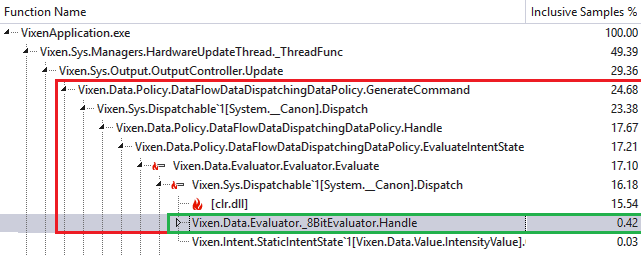
\includegraphics[width=0.85\columnwidth]{Figs/vixen_perf_original.png}
  \caption{\footnotesize \ca{Call tree} analysis of Vixen update threads}
  \label{fig:vixen_perf_original}
\end{figure}

\begin{figure}[!t]
  \centering
  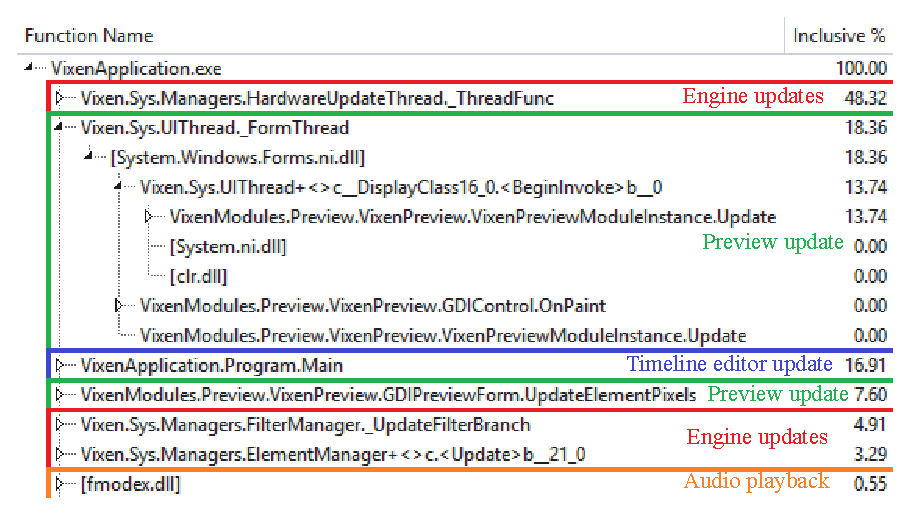
\includegraphics[width=0.85\columnwidth]{Figs/vixen_perf_original_overview.eps}
  \caption{\footnotesize \ca{Call tree} analysis of original Vixen application}
  \label{fig:vixen_perf_original_overview}
\end{figure}

The translation layers are used for determining the actual controller command format. There are several different command formats \ca{for various} controllers. For example, 8-bit, 16-bit or RGB channels. Therefore, the application \ca{needs} to resolve the actual types of commands for specific assignment handlers from a common command base type, which \ca{is} apparently very inefficient in C\#. This process is called \texttt{dispatch} in the source code\ca{;} it must be minimised in order to improve performance.

The implementation of \ca{the} preview display was also very inefficient, \ca{using} only software instance management and sequential rendering. It \cc{could} be improved by the utilisation of GPU through DirectX or OpenGL.

\ca{To reduce overheads, the show scheduler was used to render the sequences without preview and editor updates. The issue of significant refresh rate drop during \cc{the} first 60 seconds \cc{persisted}. Although the 20 fps controller became more \cc{stable} later, another 50 fps controller could only reach 40 fps maximum. The CPU usage was mostly around $55 \%$ to $75 \%$. \fref{fig:vixen_perf_original_scheduler} shows the detailed breakdown of CPU time spent for each tasks.}

\begin{figure}[!t]
  \centering
  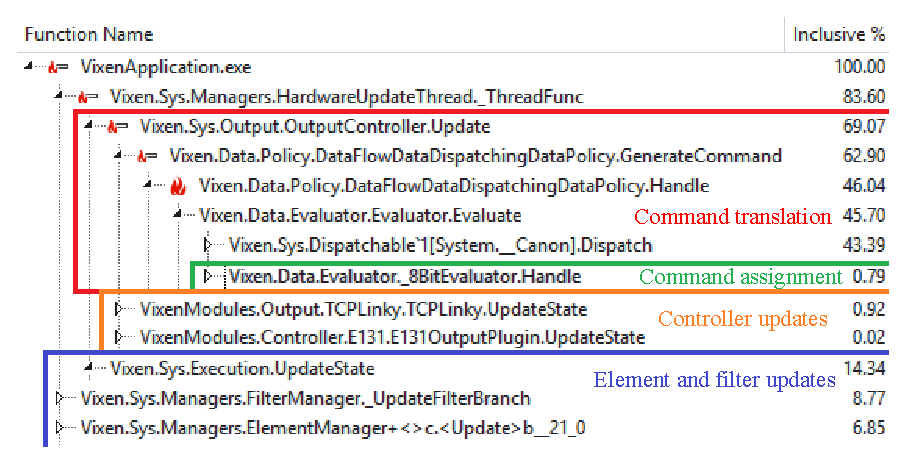
\includegraphics[width=0.85\columnwidth]{Figs/vixen_perf_original_scheduler.eps}
  \caption{\footnotesize \ca{Simplified call tree analysis of Vixen application with reduced overheads}}
  \label{fig:vixen_perf_original_scheduler}
\end{figure}

\ca{Other example sequences were also tested.} They all show similar performance characteristics with unstable playback frame \cc{rates} for moderately complicated lighting effects.

\section{Port to Linux}

It \ca{took} some necessary modifications for Vixen to run on Linux using \cc{the} mono runtime. The MonoDevelop IDE \cite{monodevelop} \ca{helped} by directly supporting Microsoft Visual Studio projects. However, C/C++ projects were not supported, and pre-built dynamic runtime libraries developed using C/C++ for Microsoft Windows were also not support by mono. All code references to WPF and FMOD audio \ca{had to be} removed for the project to build and run.

The \ca{resulting} Vixen application for Linux \cc{had} a distorted main GUI with unreasonably long vertical window size. The sequence editor, display setup and preview would either not load or crash the entire application. Fortunately, all controller modules \ca{as unmodified DLLs could} be loaded\ca{;} the core execution engine and controller update threads \ca{also} \cc{worked} properly. \fref{fig:vixen_linux_main} shows some loaded controller modules and \cc{the} partially working GUI.

\begin{figure}[!t]
  \centering
  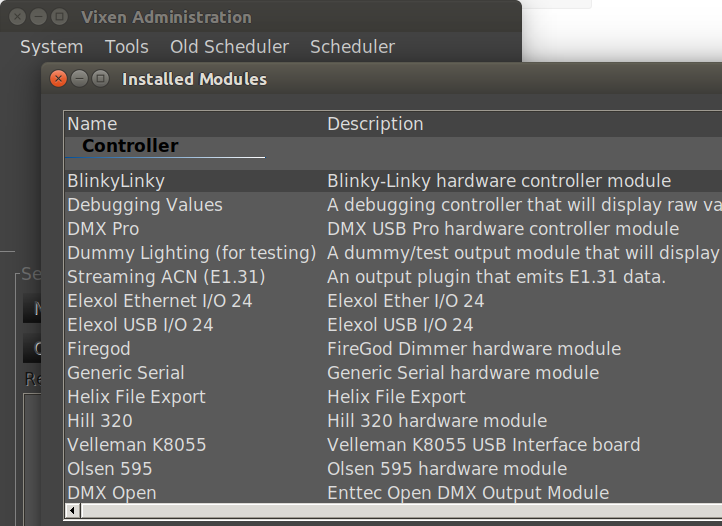
\includegraphics[width=0.8\columnwidth]{Figs/vixen_linux_controllers.png}
  \caption{\footnotesize Controller modules loaded on Linux port of Vixen application}
  \label{fig:vixen_linux_main}
\end{figure}

The intended optimised Vixen application would \cc{feature a} command-line user interface (CUI) only with minimal essential functionality. Therefore, the broken GUI should not be an issue\ca{, as \cc{GUI-related} code and modules will not be accessed in the CUI application}.

\section{\cc{Extracting} rendered sequence}

Instead of trying to improve the original execution engine, the performance problem \cc{could} be eliminated by playing pre-rendered controller layer data frames directly to individual hardware controllers. Channel data type information can be stored separately without the need to resolve through translation layers during runtime. Element updates, Filter updates, \cc{and} \ca{optional GUI updates} are all \ca{unnecessary} for \ca{rendering directly to the controllers}.

Two steps are needed for this approach. \ca{The sequence must be pre-rendered} with \cc{a} precise frame interval, then \ca{the rendered data must be played back} to the controllers as a separate process\ca{, possibly} on an entirely different platform.

To pre-render the sequence, two different methods \cc{were} possible. A dummy controller \cc{could} be used for runtime data dumping, or a separate export engine with manual frame control independent of wall-clock time \ca{\cc{could} be used}. \ca{Both of these methods were tested. Although a custom controller \cb{module \cc{could} be installed} more naturally and \cc{would} requires less modification to the existing structure, it \cc{could not} give the indication of sequence start, end and information about other controllers. More importantly, it \cc{could} have unstable frame rates influenced by CPU usage. A \cc{high-performance} computer \cc{would be} required for \cc{near-prefect} pre-rendering by controller dumping. Therefore, the existing sequence export function from \cc{the} sequence editor was used instead.}
